\chapter{Social Engineering}
First of all, we should dead with what sociology really is, then we
will master the vocabulary to be able to put a name on phenomenons,
and then we will deal with social engineering.
\section{Sociology}
Let's kick off with a definition of sociology.

\begin{boxH}
  Sociology is the \textbf{science of social phenomena} subject to
  natural and invariable laws, with the goal of discovering these
  laws.
\end{boxH}
One can quantify social interactions, and there's a cause and effect 
relationship between social phenomena.

Social sciences work on uncertain data.

\subsection{Basic Sociological Vocabulary}

Sociology uses specific terms to describe the elements of society and
social behavior. Below are key concepts:

\textbf{Norms} are the rules and expectations by which a society
guides the behavior of its members.

\textbf{Values} refer to collective ideas about what is good,
desirable, and proper.

\textbf{Role} encompasses the set of norms, behaviors, and
expectations associated with a particular social status or position
within society. Roles guide how individuals are supposed to act and
interact with others in specific contexts.

\textbf{Social Structure} is the organized pattern of social
relationships and social institutions that together constitute
society.

\textbf{Culture} consists of shared beliefs, values, and practices.


\begin{figure}[H]
  \centering
  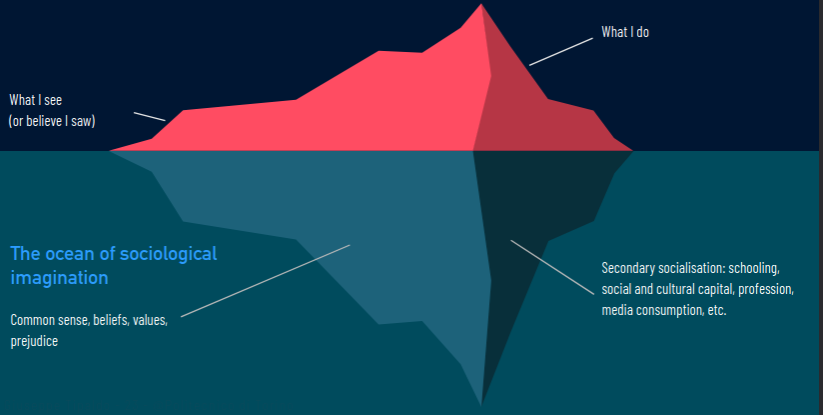
\includegraphics[width=0.5\textwidth]{img/sociology iceberg.png}
\end{figure}


